\chapter{Experiments}\label{chap:experiments}
In this Section, we define metrics to characterize the performance first in the Gazebo simulation framework, followed by the results on the \ac{AGV}. Using the Gazebo environment, we identify the required delay compensation scheme, the appropriate trajectory references and their weighting, and also the more advantageous formulation of the geometric footprint.  

\section{Performance Indicators}\label{expr_KPI}
For the task at hand, we define the following scalar metrics to highlight desirable performance traits of the controller, and where it has room for improvement, for the measurement sample size M.

\subsection{Center line deviation}
Capitalizing on the availability of the state $n$ to indicate the \ac{AGV} deviation from the reference track, we use it to measure the geometric constraint linearization for the previously introduced \ac{OCP} variants. The average centre-line deviation is subsequently defined as

\begin{align}
    \varepsilon_{n,  \mathrm{avg}} = \dfrac{1}{M}\sum_{l=0}^{M} |n_{l}|.
\end{align}

\subsection{Oscillatory measure}
Here we introduce a measure of oscillation of an arbitrary quantity $z$, which proves useful to compare the performance of different schemes for reference trajectory, and obstacle formulations. 
The second derivative approximation of this quantity is defined as

\begin{align}
    \varepsilon_{z, \mathrm{osc}} = \sqrt{\dfrac{1}{M-2}\sum_{l=0}^{M-2} (z_{l+1} - 2z_{l} + z_{l-1})^2}.
\end{align}

\section{Simulation}\label{expr_gazebo}
The physics engine Gazebo is used to develop and test the controller with a high-fidelity model before moving to the test vehicle, on an Intel i7 8850H @ 2.6 Ghz computer. In this environment, a realistic \ac{AGV} footprint is factored in along with the forces of gravity, friction and other contact forces.
This environment is interfaced with the \ac{ROS} Noetic framework, for which the \ac{MPC} controller is developed as an independent node using the python acados Application Programming Interface (API). Within this node, the previously formulated OCPs are solved approximately, with the RTI scheme in the following tests, to ensure real-time feasibility.
The application stack within which the \ac{MPC} node is encapsulated, utilizes the Hector \ac{SLAM} node for \ac{ROS}, providing localization data similar to the \ac{AGV}, that proves beneficial for tuning the controller. Another advantage of the available coupling between the application software and the physical model is that a close imitation of the delay paths can be factored into the model for optimal performance.

\begin{figure}[h!tbp]
    \begin{center}
        \def\svgwidth{1.0\textwidth}
        \input{../figures/agv_on_track.pdf_tex}
        \caption{Test track at ek robotics \cite{malitzky_markus_mechanical_nodate}.}
        \label{test_track}
    \end{center}
\end{figure}

\subsection{Trajectory reference}\label{comp_ref}

The quadratic objective function tracking the reference $s_{k, \mathrm{ref}}$ chosen just beyond reach as in \cite{kloeser_nmpc_2020} proves sufficient for the motion control task, but choppy due to the thresholding discussed in Section \ref{appr_oper_safe}:
\begin{align}
    s_{k, \mathrm{ref}} &= s_{0} + \dfrac{s_{\mathrm{ref}}}{N}\,k \label{eq_s_ref}\\
    v_{k, \mathrm{ref}} &= v_{\mathrm{ref}} \label{eq_v_ref}.
\end{align}

\begin{figure}[h!tbp]
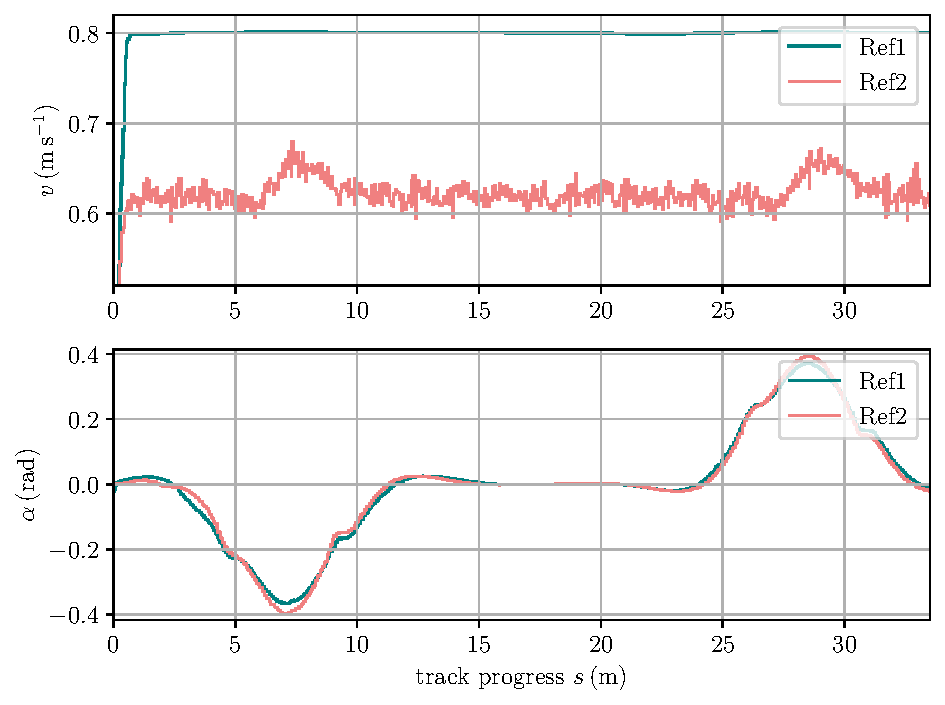
\includegraphics[width=1\textwidth]{figures/experiments/ucomp_ref}
\caption{Comparison of the impact of the application software's control thresholding for different reference trajectory schemes.} \label{fig_ucomp_ref}
\end{figure}
\begin{table}[h!tbp]
    \small
	\begin{center}
        \begin{tabular}{lccccl}\toprule
		    & \textbf{Ref1} & \textbf{Ref2}\\
            \midrule
            $\varepsilon_{v, \mathrm{osc}} $ & 4.26 $\cdot$ $10^{-3}$ $\mathrm{m\,s^{-1}}$& 2.59 $\cdot$ $10^{-2}$ $\mathrm{m\,s^{-1}}$\\
            $R$ & [ $5$, 2.5 $\cdot$ $10^{1}$ ] & [ $5$, 2.5 $\cdot$ $10^{1}$ ]\\
            $Q_{N}$ & [ $10^{-1}$, 2.5 $\cdot$ $10^{1}$, $10^{-8}$, $10^{-8}$, $5$ ] & [ $10^{-1}$, 2.5 $\cdot$ $10^{1}$, $10^{-8}$, $10^{-8}$, $5$ ]\\
            $Q$ & [ $10^{-8}$, 2.5 $\cdot$ $10^1$, $10^{-8}$, $10^{2}$, 10 ] & [ $10^{2}$, 2.5 $\cdot$ $10^1$, $10^{-8}$, $10^{-8}$ ] \\
		    \bottomrule
		\end{tabular}
	\end{center}
    \caption{Parameters of trajectory references with weighting matrices in SI units}
    \label{weight_ref}
\end{table}
The implicit velocity reference introduced Equation (\ref{eq_s_ref}) intended at progress maximization is unmerited in our case where the vehicles move on a dynamic warehouse floor, where time optimality does not take the highest priority. Instead, we introduce an explicit velocity reference in Equation (\ref{eq_v_ref}) only augmented by the former on the terminal shooting node to nudge the solution in the right direction at startup.
\par The superiority of the latter is seen in Figure \ref{fig_ucomp_ref} for this setup achieved by the state weights specified in Table \ref{weight_ref}. Another advantage of the explicit velocity reference is the geometric constraint simplification discussed in Section \ref{safety_field}.
\subsection{Delay compensation}\label{expr_del_comp}

\par Since the application layer is aware of the true applied input $\tilde{\zeta}^{u}$, unlike the MPC, three delay compensation schemes are investigated here for the round trip delay $\tau_{rt}$ as $\tau_{rt}$ = $\tau_{c}$ + $\tau_{a}$ + $\tau_{m}$. The first, referred to as $\mathrm{Eu}\,2$, relies on the delay compensation block in the application to account for $\tau_{m}$ + $\tau_{a}$, and the remaining delay compensation from the \ac{MPC} layer itself. In the second scheme i.e the $\mathrm{Eu}\,1$, the Euler predictor in the application compensates $\tau_{m}$, and $\tau_{c}$ + $\tau_{a}$ is compensated by forward simulating with the \ac{RK}4 integrator in the proposed controller. The third scheme, $\mathrm{Eu}\,0$ refers to complete $\tau_{rt}$ compensation in the \ac{MPC} layer. 

\begin{figure}[h!tbp]
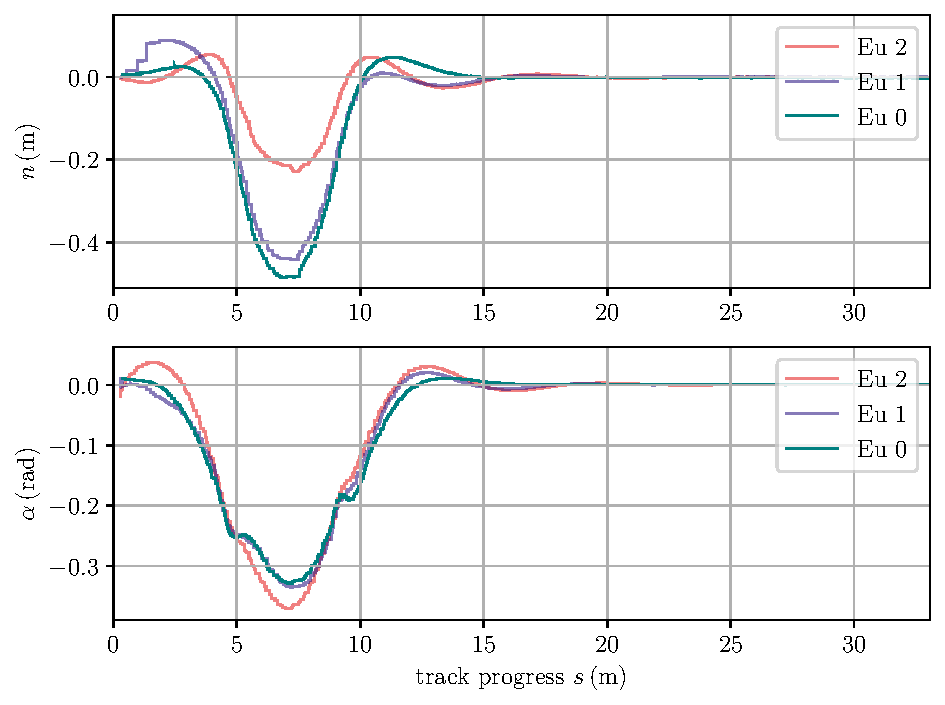
\includegraphics[width=1\textwidth]{figures/experiments/predictor}
\caption{Overshoot comparison of delay compensation schemes.}\label{fig1_comp_pred}
\end{figure}

\par After the right-hand curve on the track from $s$ = 7.5 m to $s$ = 10 m indicated in Figure \ref{test_track}, we see the decay of $n$ is marginally better with the $\mathrm{Eu}\,0$ in Figure \ref{fig1_comp_pred}. Despite the concern that the $\mathrm{Eu}\,0$ is agnostic to the applied vector $\tilde{\zeta^{u}}$ discussed in Section \ref{appr_oper_safe} that could lead to loss of solution robustness, the results discussed in Section \ref{comp_ref} with the explicit velocity reference assure us of the inactive control thresholding.
\par Thus, the sufficiency of the delay compensation purely in the \ac{MPC} layer is justified by experimental validation using the states $n$, $\alpha$.


\subsection{Direct and lifted formulations for the AGV elliptical footprint}

\begin{figure}[h!tb]
    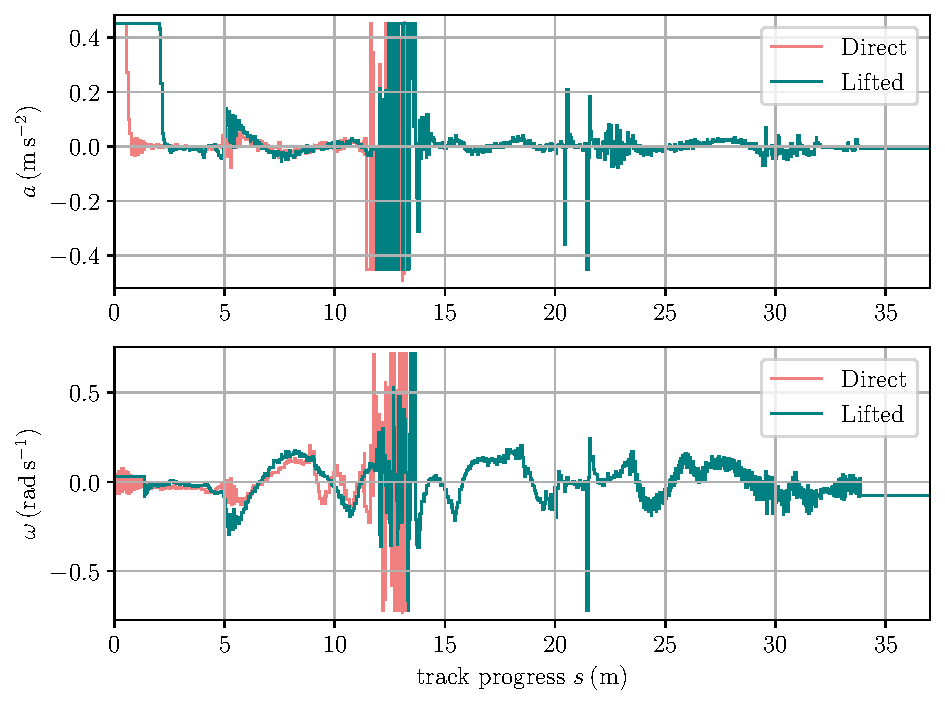
\includegraphics[width=1\textwidth]{figures/experiments/u_2c}
    \caption{Control $u$ comparison for the \ac{AGV} elliptical footprint and circular obstacles formulation in Gazebo.}  \label{fig_comp_u_2c}
\end{figure}

\begin{table}[h!tb]
    \small
	\begin{center}
        \begin{tabular}{lccccl}\toprule
		    & \textbf{Direct} & \textbf{Lifted}\\
            \midrule
            $\varepsilon_{a,\,\mathrm{osc}} $ & 7.95 $\cdot$ $10^{-1}\,\mathrm{m\,s^{-2}}$& 2.67 $\cdot$ $10^{-1}\,\mathrm{m\,s^{-2}}$\\
            $\varepsilon_{\omega,\,\mathrm{osc}} $ & 9.90 $\cdot$ $10^{-1}\,\mathrm{rad\,s^{-1}}$& 1.78 $\cdot$ $10^{-1}\,\mathrm{rad\,s^{-1}}$\\
		    \bottomrule
		\end{tabular}
	\end{center}
    \caption{Control oscillation metrics for the \ac{AGV} elliptical footprint and circular obstacles formulation in Gazebo.}
    \label{tab_u_osc_2c}
\end{table}

In this section, we inspect the solution trajectories of the \ac{OCP}s mentioned in Section \ref{appr_fren_traj} for the elliptical \ac{AGV} footprint. 
In order to achieve an unbiased comparison of the two trajectory tracking controllers with obstacle avoidance, we eliminate the drift of the obstacle state estimated by the \ac{KF} by assuming perfect knowledge of its position and dimensions.
As indicated previously in Section \ref{appr_footprint}, the elliptical \ac{AGV} footprint is a severely nonlinear function of the state $\zeta^{c}$, which can be seen in the poor convergence of the control trajectory $u$ in Figure \ref{fig_comp_u_2c}, for the direct elimination and lifted formulations.
Burdened with the additional nonlinearity introduced in the geometric constraint of the direct elimination formulation due to the nonlinear projection defined in Equation (\ref{F2C}), the simulated \ac{AGV} fails to maneuver around the first circular obstacle at $s$ = 13, where the solution stagnates at the poor local optima. Despite the lifted controller completing the track, we disqualify it from subsequent vehicle tests due to the poor quality of the controls. 

% \begin{figure}[h!tb]
%     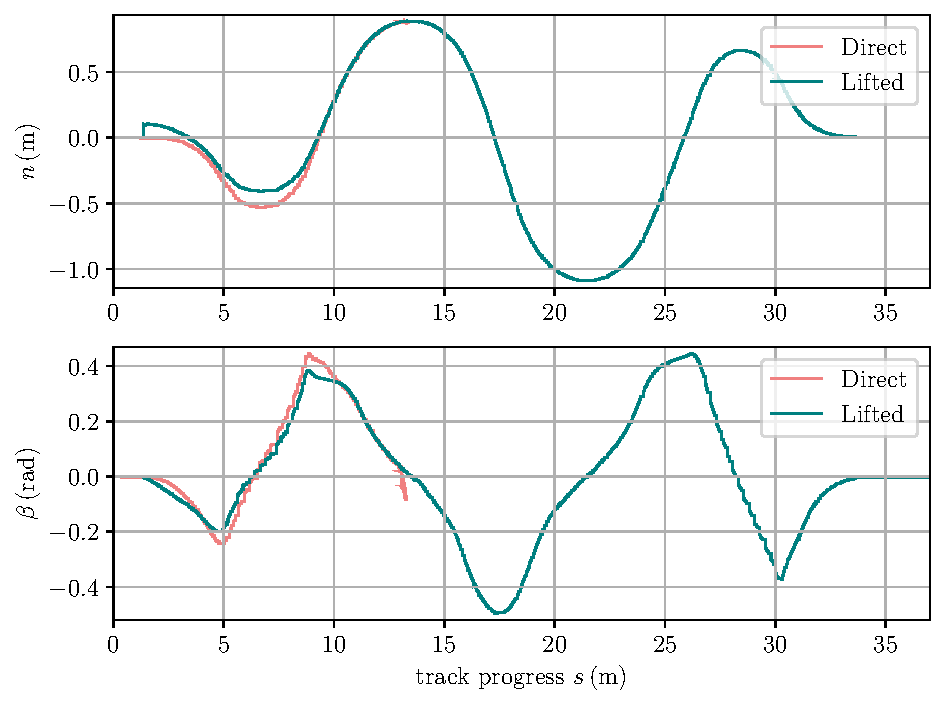
\includegraphics[width=1\textwidth]{figures/experiments/zeta_f_2c}
%     \caption{State $\zeta^{f}$ comparison from the closed loop Gazebo tests.}  \label{fig_comp_zeta_f}
% \end{figure}

\begin{figure}[h!tb]
    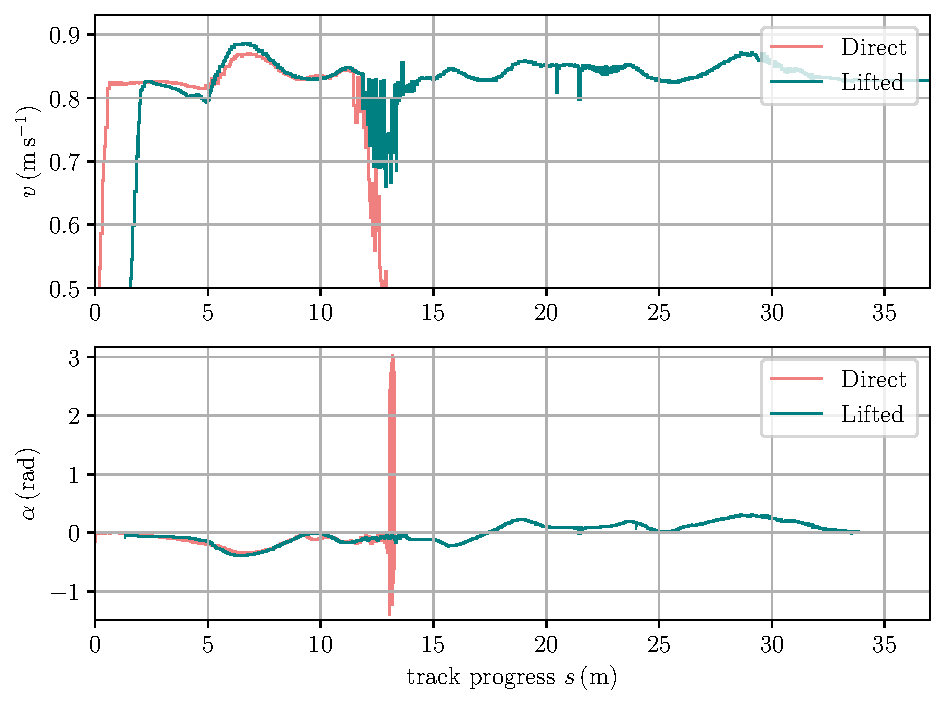
\includegraphics[width=1\textwidth]{figures/experiments/zeta_u_2c}
    \caption{State $\zeta^{u}$ comparison for the \ac{AGV} elliptical footprint and circular obstacles formulation in Gazebo.}  \label{fig_comp_zeta_u_2c}
\end{figure}

\begin{figure}[tb]
    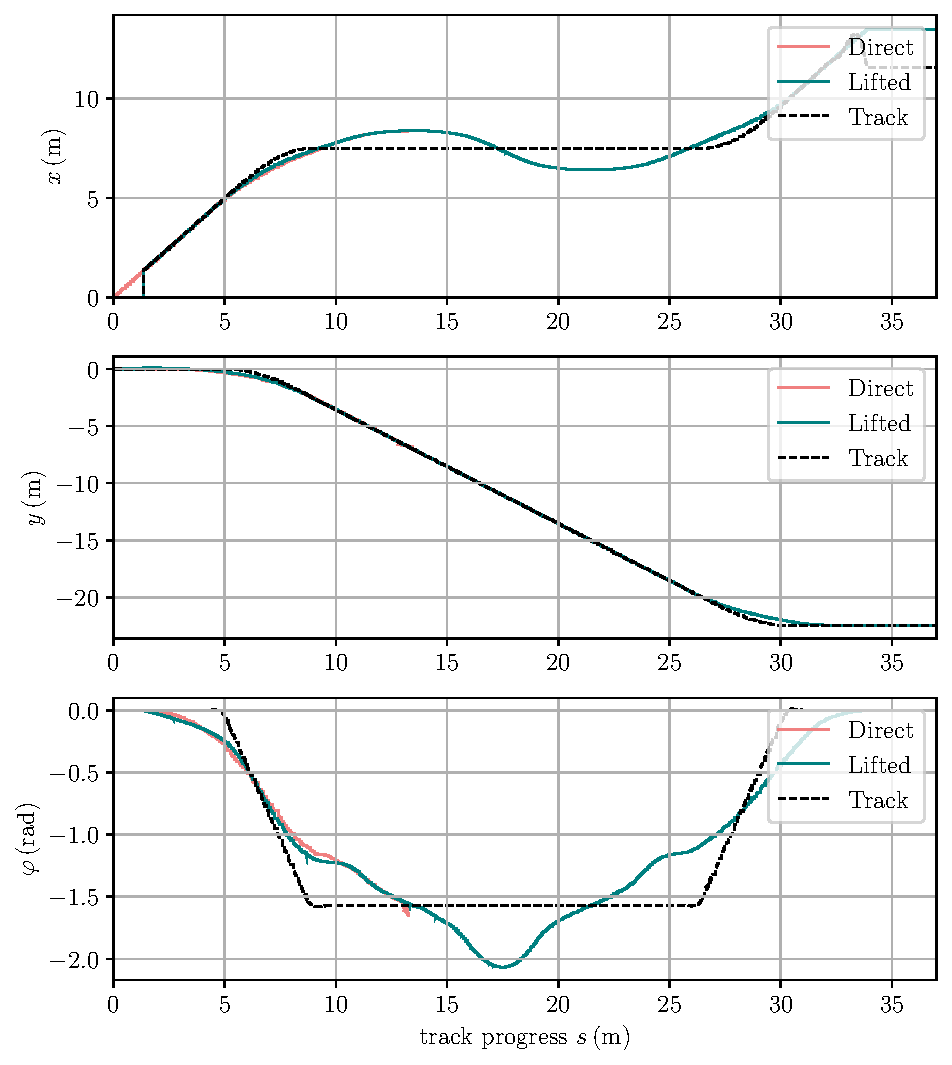
\includegraphics[width=1\textwidth]{figures/experiments/zeta_c_2c}
    \caption{State $\zeta^{c}$ comparison for the \ac{AGV} elliptical footprint and circular obstacles formulation in Gazebo.}  \label{fig_comp_zeta_c_2c}
\end{figure}
\newpage
% \newpage
\clearpage

\subsection{Direct and lifted formulations for the AGV covering circles}

\begin{figure}[h!tb]
    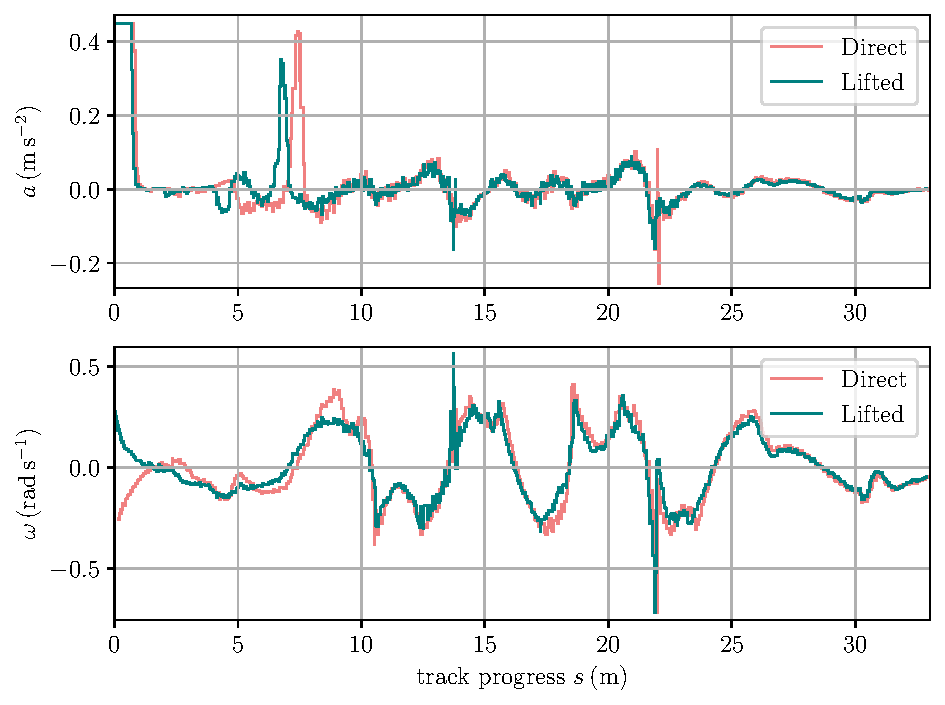
\includegraphics[width=1\textwidth]{figures/experiments/u}
    \caption{Control $u$ comparison for the \ac{AGV} covering circles and elliptical obstacles formulation in Gazebo.}  \label{fig_comp_u}
\end{figure}
\begin{table}[h!tb]
    \small
	\begin{center}
        \begin{tabular}{lccccl}\toprule
		    & \textbf{Direct} & \textbf{Lifted}\\
            \midrule
            $\varepsilon_{a,\,\mathrm{osc}} $ & 1.58 $\cdot$ $10^{-2}\,\mathrm{m\,s^{-2}}$& 1.56 $\cdot$ $10^{-2}\,\mathrm{m\,s^{-2}}$\\
            $\varepsilon_{\omega,\,\mathrm{osc}} $ & 1.57 $\cdot$ $10^{-2}\,\mathrm{rad\,s^{-1}}$& 2.25 $\cdot$ $10^{-2}\,\mathrm{rad\,s^{-1}}$\\
		    \bottomrule
		\end{tabular}
	\end{center}
    \caption{Control oscillation metrics for the \ac{AGV} covering circles and elliptical obstacles formulation in Gazebo.}
    \label{tab_u_osc_2el}
\end{table}

In this section, we proceed with the Gazebo tests for the covering circles, again under the assumption of no drift in the obstacle estimation. Observing the feasibility of both controllers for the task at hand, we carefully inspect the state and controls, with respect to the previously defined metrics.

\begin{figure}[h!tb]
    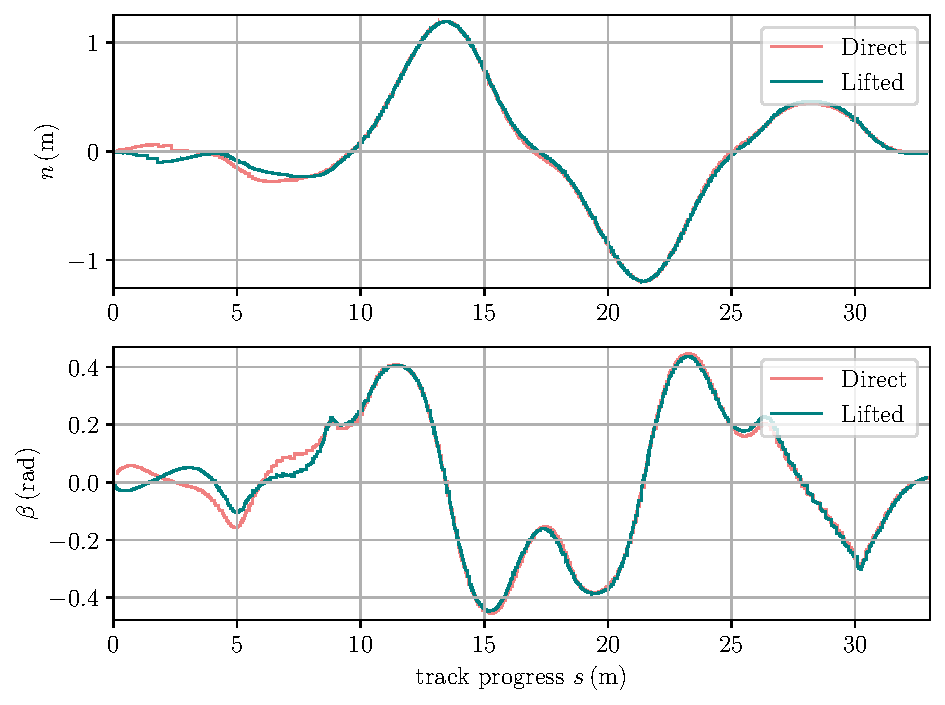
\includegraphics[width=1\textwidth]{figures/experiments/zeta_f}
    \caption{State $\zeta^{f}$ comparison for the \ac{AGV} covering circles and elliptical obstacles formulation in Gazebo.}  \label{fig_comp_zeta_f}
\end{figure}

\begin{figure}[h!tb]
    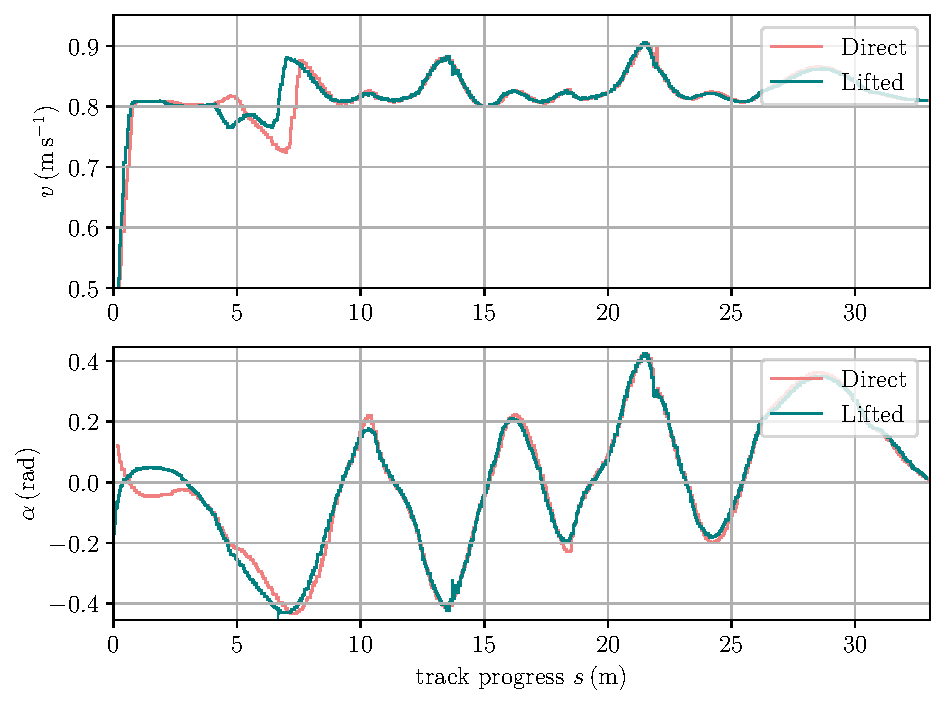
\includegraphics[width=1\textwidth]{figures/experiments/zeta_u}
    \caption{State $\zeta^{u}$ comparison for the \ac{AGV} covering circles and elliptical obstacles formulation in Gazebo.}  \label{fig_comp_zeta_u}
\end{figure}

\begin{figure}[h!tb]
    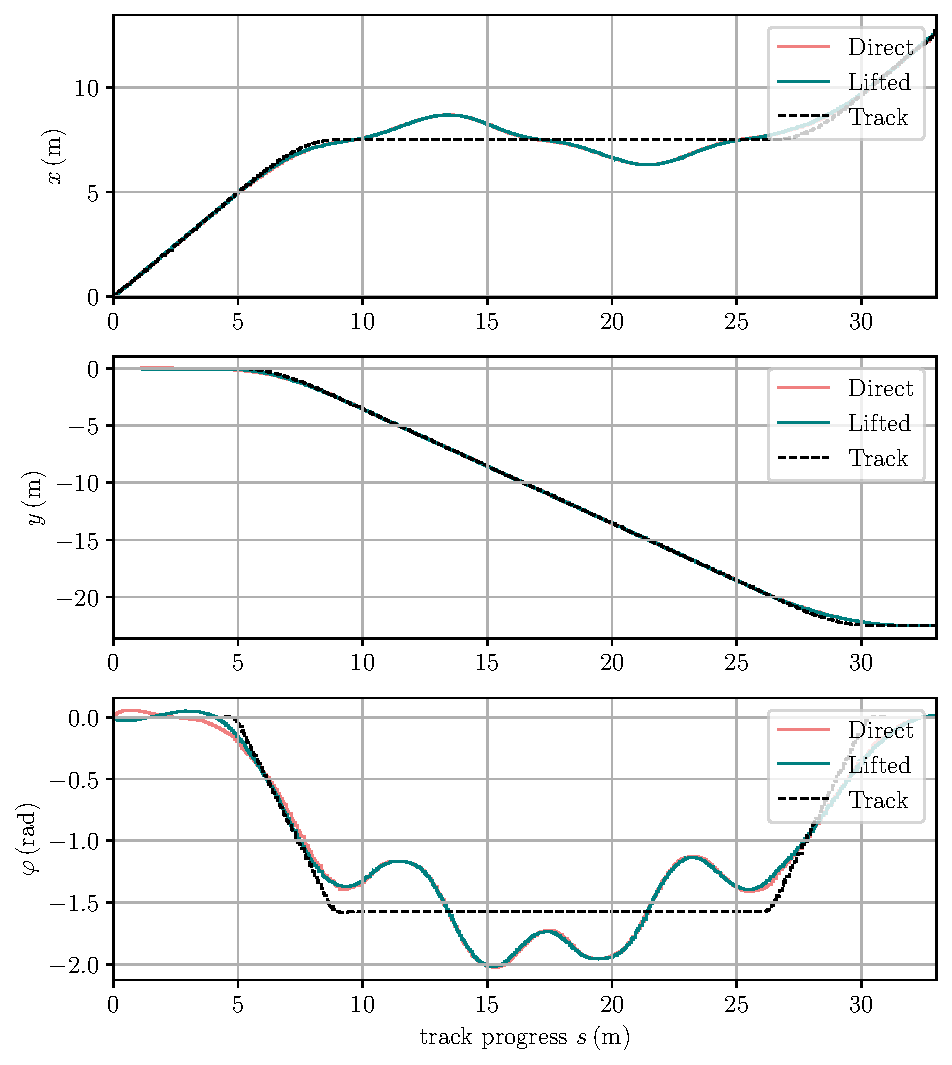
\includegraphics[width=1\textwidth]{figures/experiments/zeta_c}
    \caption{State $\zeta^{c}$ comparison for the \ac{AGV} covering circles and elliptical obstacles formulation in Gazebo.}  \label{fig_comp_zeta_c}
\end{figure}

\begin{figure}[h!tb]
    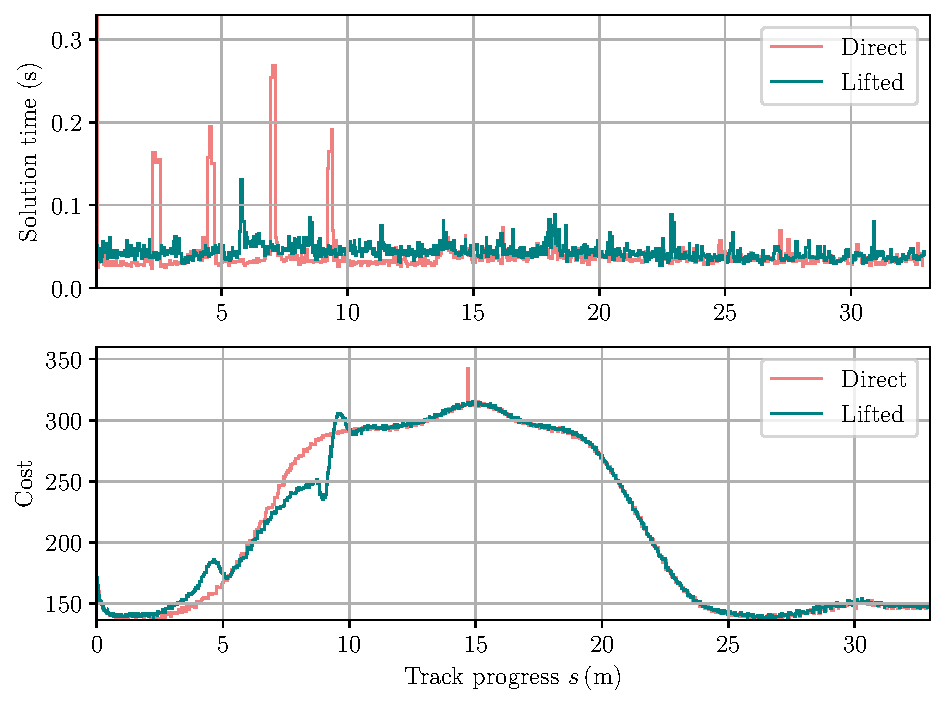
\includegraphics[width=1\textwidth]{figures/experiments/metrics}
    \caption{Solution comparison for the \ac{AGV} covering circles and elliptical obstacles formulation in Gazebo.}  \label{fig_metrics}
\end{figure}

\begin{table}[h!]
    \small
	\begin{center}
        \begin{tabular}{lccccl}\toprule
		    & \textbf{Direct} & \textbf{Lifted}\\
            \midrule
            $\varepsilon_{n,\,\mathrm{avg}} $ & 5.10 $\cdot$ $10^{-1}$ m& 5 $\cdot$ $10^{-1}$ m\\
            $\tau_{\mathrm{rti,\,avg}} $ & 3.99 $\cdot$ $10^{-2}$ s& 4.39 $\cdot$ $10^{-2}$ s\\
            $\tau_{\mathrm{rti,\,max}} $ & 2.69 $\cdot$ $10^{-1}$ s& 1.34 $\cdot$ $10^{-1}$ s\\
		    \bottomrule
		\end{tabular}
	\end{center}
    \caption{Centreline deviation and solution times for the \ac{AGV} covering circles and elliptical obstacles formulation in Gazebo.}
    \label{tab_rti_sim}
\end{table}

Both formulations tested here complete the track with similar solution trajectories as indicated in Figures \ref{fig_comp_zeta_c}, \ref{fig_comp_zeta_f}, \ref{fig_comp_zeta_u}, and \ref{fig_comp_u} with minor differences in solution times. These differences, however, are significant in evaluating real-time feasibility of the proposed optimal control schemes. In Figure \ref{fig_metrics}, we observe that, although the direct elimination formulation has a lower average SQP solution time $\tau_{\mathrm{rti,\,avg}}$, it exceeds the MPC assigned computation deadline $\tau_{c}$ several times. Since the drive controller applies the previous control in this scenario, the guarantee of overall solution optimality is lost, despite retaining the feasibility of the trajectory tracking problem.
\goodbreak
\newpage
% \newpage
\clearpage

\section{Warehouse tests}

Both formulations are tested with cylindrical and cuboidal obstacles, with the \ac{AGV} covering circles formulation along the track at the warehouse, similar to the one previously described in the Gazebo simulation. The track begins with a right-hand curve followed by a $20 \mathrm{m}$ long straight path and ends with a left curve. The obstacles are placed at $s$ = $13 \mathrm{m}$ and $s$ = $17\mathrm{m}$ offset by $n$ = $0.25 \mathrm{m}$ and $n$ = $-0.25 \mathrm{m}$ respectively from the centre line. The unreliability of obstacle detection with the laser scanner's limited field of view aboard the \ac{AGV} is further exacerbated by the need to exclude vehicle chassis reflections. To avoid the \ac{AGV} footprint being considered as an active constraint, leading to infeasibility, a minimal angle is used in conjunction with the \ac{KF} to estimate the occluded objects during maneuvres. The closed-loop trajectories of state and control of the lifted formulation are presented in Figures \ref{fig_zeta_time} and \ref{fig_u_time}.
\par We continue to use the RTI scheme as in simulation, to solve the \ac{OCP}s aboard the \ac{AGV}, which is equipped with an industrial computer running the \ac{ROS} Noetic framework for Ubuntu on an Intel i7 9700TE @ 1.8 Ghz. The $\tau_{\mathrm{rti,\,avg}}$ indicates that the solution times are well within the soft deadline $\tau_{c}$ of the MPC node during the remainder of the tracking, proving its feasibility. Additionally, comparing the obtained SQP solution times in Tables \ref{tab_rti_sim} and \ref{tab_rti_agv}, the lower average SQP solution times for both formulations on the vehicle strengthens the argument that the lifted formulation is en route to real-time optimal performance.
\begin{figure}[h!tb]
    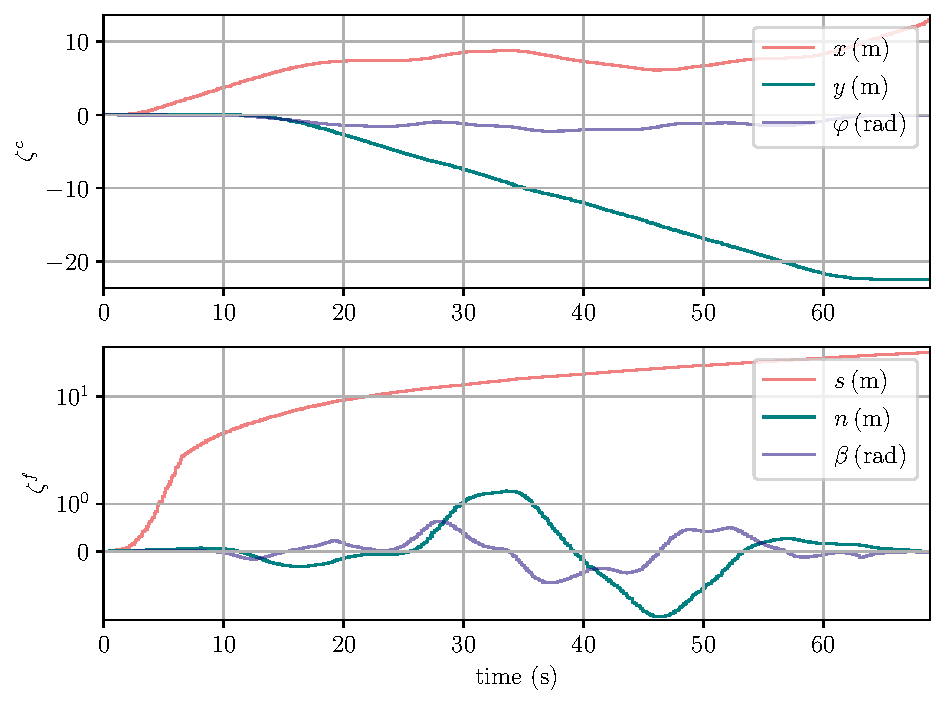
\includegraphics[width=1\textwidth]{figures/experiments/zeta_time}
    \caption{State $\zeta^{l}$ for the lifted formulation with \ac{AGV} covering circles and elliptical obstacles from the real warehouse.}  \label{fig_zeta_time}
\end{figure}
\begin{table}[tb]
    \small
	\begin{center}
        \begin{tabular}{lccccl}\toprule
		    & \textbf{Direct} & \textbf{Lifted}\\
            \midrule
            $\varepsilon_{n, \mathrm{avg}} $ & 3.828 $\cdot$ $10^{-1}$ m& 4.688 $\cdot$ $10^{-1}$ m\\
            $\tau_{\mathrm{rti,\,avg}} $ & 2.899 $\cdot$ $10^{-2}$ s& 3.099 $\cdot$ $10^{-2}$ s\\
		    \bottomrule
		\end{tabular}
	\end{center}
    \caption{Centreline deviation and average solution time for the \ac{AGV} covering circles and elliptical obstacles formulation in the real warehouse.}
    \label{tab_rti_agv}
\end{table}
\begin{table}[h!]
    \small
	\begin{center}
        \begin{tabular}{lccccl}\toprule
		    & \textbf{Direct} & \textbf{Lifted}\\
            \midrule
            $\varepsilon_{v,\,\mathrm{osc}} $ & 7.96 $\cdot$ $10^{-2}\,\mathrm{m\,s^{-1}}$& 4.37 $\cdot$ $10^{-2}\,\mathrm{m\,s^{-1}}$\\
            $\varepsilon_{a,\,\mathrm{osc}} $ & 5.69 $\cdot$ $10^{-2}\,\mathrm{m\,s^{-2}}$& 9.52 $\cdot$ $10^{-2}\,\mathrm{m\,s^{-2}}$\\
            $\varepsilon_{\omega,\,\mathrm{osc}} $ & 1.66 $\cdot$ $10^{-1}\,\mathrm{rad\,s^{-1}}$& 2.86 $\cdot$ $10^{-1}\,\mathrm{rad\,s^{-1}}$\\
		    \bottomrule
		\end{tabular}
	\end{center}
    \caption{Control oscillation metrics for the \ac{AGV} covering circles and elliptical obstacles formulation in the real warehouse.}
    \label{tab_u_osc_agv_2el}
\end{table}
\begin{figure}[h!]
    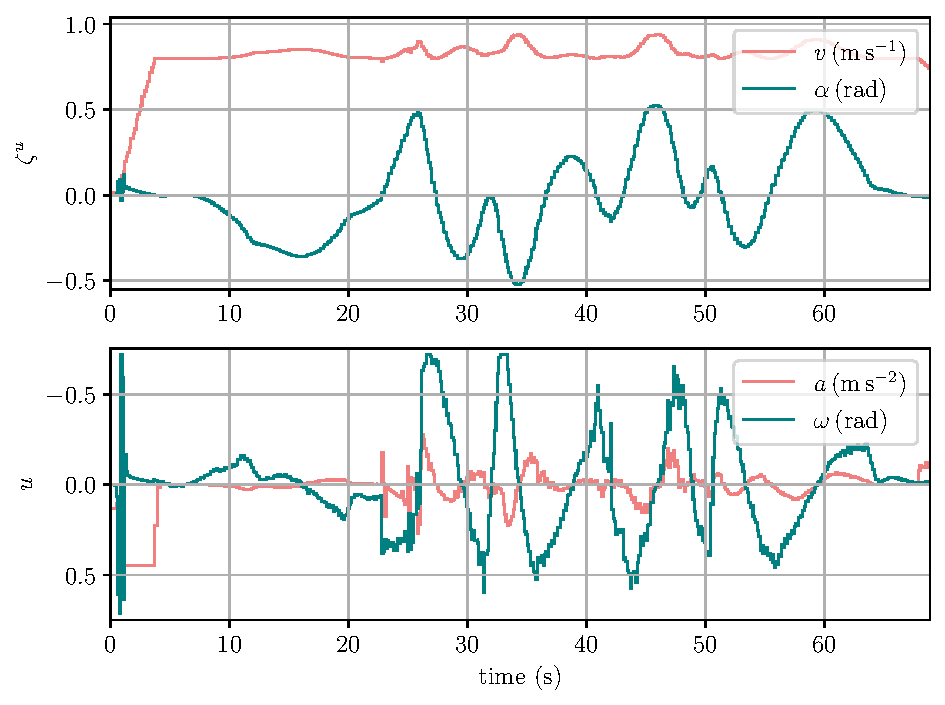
\includegraphics[width=1\textwidth]{figures/experiments/u_time}
    \caption{Control $u$ for the the lifted formulation with \ac{AGV} covering circles and elliptical obstacles from the real warehouse.}  \label{fig_u_time}
\end{figure}